对于 SFibAI、w/o View、w/o Weak Loc.\ 和完整 VCRE-Fib，验证集所选 epoch 分别为 65、80、39、47，$\risk$ 为 0.172661、0.157844、0.159315、0.156067。验证集含 20,880 张图像、1,227 名患者和 33 个中心。附录表~\ref{tab:freeze} 记录四个冻结检查点，图~\ref{fig:training} 展示相同 90 epoch 上限下的四条训练轨迹。这些记录交代检查点选择来源，模型的观测排序仍由测试集主终点确定。
\inputtable{tab10_freeze}
四模型均用四 GPU、SyncBatchNorm 和全局 batch 24，共同训练设置见附录~\ref{sec:appendix-implementation}。在验证集上从第 21--90 epoch 中依次按较低 $\risk$、较低 image COR、较早 epoch 的顺序选择检查点，并在测试集评价前冻结。图~\ref{fig:training} 展示全部 90 个逐轮记录，未作平滑。各模型总损失包含不同的辅助项，用于模型内部训练诊断。图~\ref{fig:losses} 展示完整模型的损失分项。
\begin{figure}[!htbp]
\centering
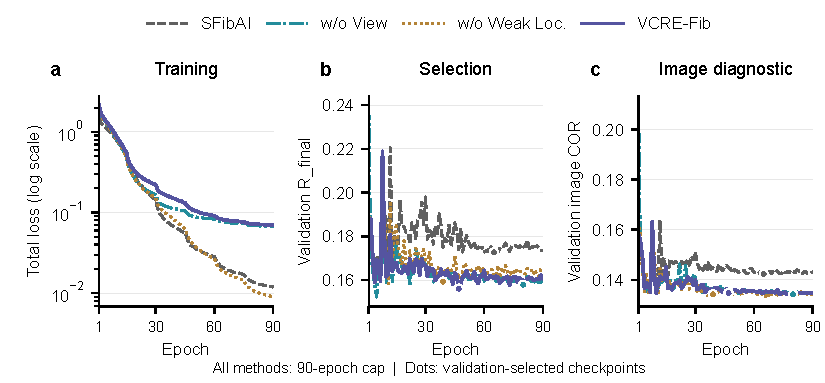
\includegraphics[width=\linewidth]{figures/assets/training_curves.pdf}
\caption{\lang{Training and validation trajectories under a common 90-epoch cap. (a) Total training loss on a logarithmic axis, including each model's auxiliary terms. (b) Validation $R_{\mathrm{final}}$. (c) Validation image COR. Curves show unsmoothed epoch-level observations; dots mark the validation-selected checkpoints in Table~\ref{tab:freeze}.}{统一 90 epoch 上限下的训练与验证集轨迹。(a) 含各模型辅助项的训练总损失，纵轴为对数尺度。(b) 验证集 $R_{\mathrm{final}}$。(c) 验证集 image COR。曲线为未经平滑的逐轮观测，圆点标记表~\ref{tab:freeze} 中由验证集选择的检查点。}}\label{fig:training}
\end{figure}

\begin{figure}[!htbp]
\centering
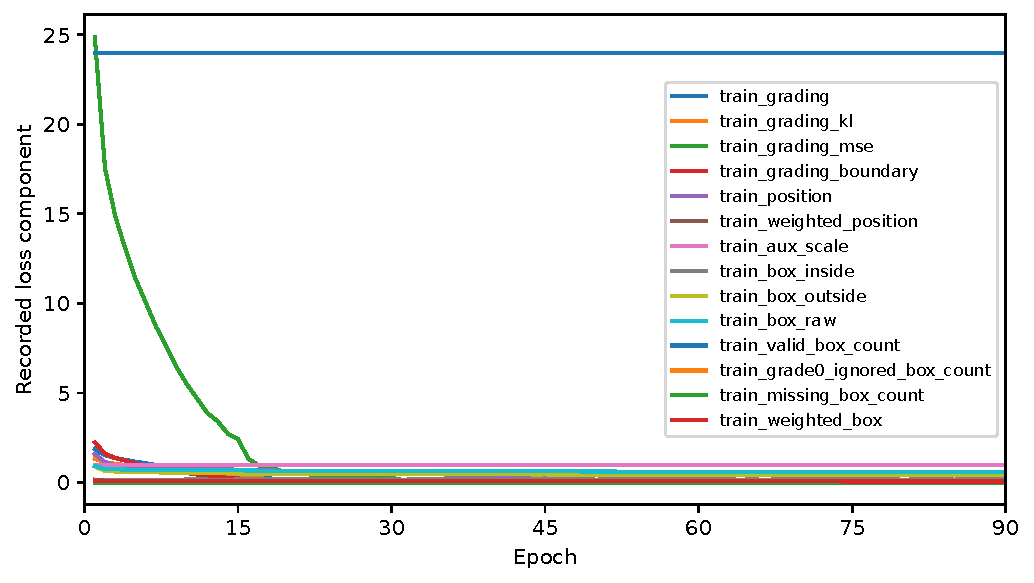
\includegraphics[width=\linewidth]{figures/assets/synap_loss_components.pdf}
\caption{\lang{Full VCRE-Fib loss components under the same 90-epoch cap, shown as training diagnostics rather than estimates of module effects.}{完整 VCRE-Fib 在相同 90 epoch 上限下的训练损失分项，用于训练诊断，不作为模块效应估计。}}\label{fig:losses}
\end{figure}

\FloatBarrier
